\documentclass[journal,10pt,onecolumn,compsoc,letterpaper,draftclsnofoot,table,xcdraw]{IEEEtran} \usepackage[margin=0.75in]{geometry}
\usepackage{pdfpages}
\usepackage{minted}
\usepackage{graphicx,float} 
\usepackage{listings}
\usepackage{verbatim}
\usepackage{url}
\usepackage{nameref}
\usepackage{setspace} \singlespacing
\graphicspath{/graphics} \setlength{\parskip}{\baselineskip} \setlength\parindent{24pt}
\usepackage[english]{babel}
\usepackage{fullpage}
\usepackage{hyperref}
\hypersetup{
    colorlinks,
    citecolor=black,
    filecolor=black,
    linkcolor=black,
    urlcolor=black
}
\title{Project 2: I/O Elevators}
\author{Group 10-03: Behnam Saeedi, zhaoheng wang, Levi Willmeth\\ CS444: Operating systems II}
\date{\today}
\begin{document}
\maketitle
\begin{centering}
Spring 2017
\begin{abstract}
\noindent The purpose of this homework is to get familiar with I/O schedulers and how they work. During the course of this assignment we will cover implementation of Look scheduler. Furthermore, we will discuss its properties, implementation and features. Furthermore, we will answer the provided questions in the assignment description. Next, we will cover the dining philosopher problem and our solution to it. Finally we will go over the work log and and the contribution of members to git repository for this assignment. This data will be represented in a table format.
\end{abstract}
\end{centering}
%--------------------------------------------------------------
\newpage
\tableofcontents
\newpage 
%--------------------------------------------------------------
\section{Look}
\subsection{Look ahead}
Look scheduler introduces a method of feeding the data to the memory by optimizing the movement of the read write head and reducing random movements. The reason to such a naming is the "Look ahead" functionality. The way this algorithm works is that it will process the orders by looking ahead in the queue and selecting the ones that are on the way as well. From a data structural perspective, this just means that the data order is sorted based on the memory sector which it appears in.  For example, if we are at sector 50 processing orders and moving toward the higher sectors, on our move to process sector 150, we will process orders that are between 50 an 150 in an ascending order. After it processes the highest sector on the path, it switches its direction and starts processing orders sorted on descending order from 150 to 0. Again as mentioned earlier, we are essentially sorting the orders based on the 2 factors. First factor is the number of the order's sector and second factor is whether the head is moving across sectors in ascending order or descending order.
\subsection{Bias}
\noindent This approach has an interesting bias. The issue occurs when on our path new orders get placed between moving from two sectors. For example, lets assume we have just processed the order at sector 50 and are moving to sector 150 for the next order. While we are moving new orders get added to sectors 58, 60, 66, 80, 96, 109, 120 and 144 which are all in between 50 and 150. Now we have process those since they are on the way. This means even though order at sector 150 appeared way before all of those 8 new orders, we do not get to process the 150 in a First In First Out (FIFO) fashion. This is know as the bias of Look scheduling algorithm.
\subsection{Complications}
\noindent This scheduler has an expensive process. It is not straight forward to calculate the order of order of operations and it requires some book keeping. Furthermore, the bias can cause some of the processes to starve. Likewise, what if we are at sector 50 moving up and there are orders at sector 49, 48 and 45. This means we are ignoring orders that could be achieved quickly and seamlessly with little effect on other processes service time.
\subsection{Variants}
\noindent The look scheduler has several variants each designed to address one or more issues that come with the look algorithm.
\subsubsection{C-Look}
\noindent C-Look or Circular look is designed to help with the complication of determining the path of the head as it moves. The C-look states that we only process lines moving in one direction and when we are done we go back to sector 1 and start over. This means if we are processing orders 50 to 150 and new order appears at order 48, we will not process that on our way back from 150 to 1, but rather we will move to sector one then we start moving in the ascending direction and process the order 48. In other words, we are only processing orders that are on our way as we are moving across sectors in  an ascending order. The reason it is called circular becomes clear when we imagine this as a sorted linked list:
\begin{table}[ht]
\centering
\caption{Illustration of Circular Look ahead algorithm for scheduler}
\label{C-Look}
\begin{tabular}{ll}
\hline
\rowcolor[HTML]{BBDAFF} 
\multicolumn{1}{|l|}{\cellcolor[HTML]{BBDAFF}Sector} & \multicolumn{1}{l|}{\cellcolor[HTML]{BBDAFF}Order} \\ \hline
\multicolumn{2}{c}{\begin{tabular}[c]{@{}c@{}}.\\ .\\ .\end{tabular}}                                     \\ \hline
\multicolumn{1}{|l|}{50}                             & \multicolumn{1}{l|}{R}                             \\ \hline
\multicolumn{2}{c}{$\uparrow$ $\downarrow$}                                                               \\ \hline
\multicolumn{1}{|l|}{87}                             & \multicolumn{1}{l|}{W}                             \\ \hline
\multicolumn{2}{c}{$\uparrow$ $\downarrow$}                                                               \\ \hline
\multicolumn{1}{|l|}{106}                            & \multicolumn{1}{l|}{W}                             \\ \hline
\multicolumn{2}{c}{$\uparrow$ $\downarrow$}                                                               \\ \hline
\multicolumn{1}{|l|}{150}                            & \multicolumn{1}{l|}{R}                             \\ \hline
\multicolumn{2}{c}{\begin{tabular}[c]{@{}c@{}}.\\ .\\ .\end{tabular}}                                    
\end{tabular}
\end{table}

\noindent According to this diagram, if we process order 150, we have to go back to sector 50 and start over which would be equivalent to wrapping the linked list around in a circle since the next order after 150 in this circular linked list is the order 50.

\subsubsection{ F-Look, N-Look}
\noindent As we mentioned earlier, each variant solves one or more issues with Look scheduler. The N and F variants are designed to solve the problem with bias by introducing a time constraint. However, in this assignment we will not be implementing these variant.
\subsubsection{S-Look}
\noindent S-Look seeks to process the shortest order first. As we mentioned earlier in the Complications subsection, If we are moving on a pass we are ignoring all of the orders behind us regardless of how close they are. The S-Look seeks to solve this issue by introducing a shortest distance first approach. This means if an order is closer to the ahead at the opposite direction, the head will change direction. For example, if we are at position 50 and next order is at 150 and we are moving toward it, if an order appears at 45 (behind us) the head will change direction and process that one first.
\subsection{Our Implementation: C-Look}
\noindent In this assignment we tried to implement the C-Look scheduler. This scheduler will be located in:
\begin{minted}{bash}
$ linux-yocto-3.14/block/sstf-iosched.c
\end{minted}
\noindent The only function that would be affected in this file is the "add\char`_request" function. Everything else is already taken care of by other methods. The way we are implementing this section is through an insertion sort.
\begin{itemize}
\item Following steps needed to be taken for this implementation of insertion sort:
\item Create an instance of sstf\char`_data that points to the elevator data (it is called nd)
\item "nd" will contain request queue's elevator's elevator data (pointer)
\item check if the q$\rightarrow$elevator$\rightarrow$elevator\char`_data$\rightarrow$queue is empty or not
\item if it is empty or has only one member:
	\begin{itemize}
	\item add the new request to end queue list
	\end{itemize}
\item if the queue has more than 1 memeber in it:
	\begin{itemize}
	\item this means there are membesrs of queuelist available in the nd$\rightarrow$queue
    \item insert the new request in proper position:
   		\begin{itemize}
		\item Create an iterator of type request
        \item Go through each member in the nd$\rightarrow$queue that is of type queuelist
        \item Insert the new request in the list if the current position
		\end{itemize}
	\end{itemize}
\end{itemize}
\subsection{Code}
\begin{minted}{c}
/*
 * LOOK I/O scheduler for OSU CS444 Spring 2017
 * Written by Levi Willmeth, Behnam Saeedi, and Zhaoheng Wang
 */
#include <linux/blkdev.h>
#include <linux/elevator.h>
#include <linux/bio.h>
#include <linux/module.h>
#include <linux/slab.h>
#include <linux/init.h>

struct sstf_data {
	struct list_head queue;
};

static void sstf_merged_requests(struct request_queue *q, struct request *rq,
				 struct request *next)
{
	list_del_init(&next->queuelist);
}

static int sstf_dispatch(struct request_queue *q, int force)
{
	struct sstf_data *nd = q->elevator->elevator_data;

	if (!list_empty(&nd->queue)) {
		struct request *rq;
		rq = list_entry(nd->queue.next, struct request, queuelist);
		list_del_init(&rq->queuelist);
		elv_dispatch_sort(q, rq);
		return 1;
	}
	return 0;
}

static void sstf_add_request(struct request_queue *q, struct request *rq)
{
	printk(KERN_DEBUG "adding new request...\n");
	struct sstf_data *nd = q->elevator->elevator_data;
	/* checking if the queue is not empty */
	if(!list_empty(&nd->queue)) {
		printk(KERN_DEBUG "queue is not emty, generating an itterator...\n");
		/* Creatinga n itterator */
		struct request * it;
		/* create the distance indecies */
		int new_distance;
		/* Itterate: */
		list_for_each_entry(it, &nd->queue, queuelist) {
			sector_t new_sector = blk_rq_pos(rq);
			sector_t current_sector = blk_rq_pos(it);
			new_distance = new_sector - current_sector;
			printk(KERN_DEBUG "Distance is %i\n", new_distance);
			if (new_distance < 0)
				list_add_tail(&rq->queuelist, &it->queuelist);
		}
	}
	printk(KERN_DEBUG "adding to tail...\n");
	list_add(&rq->queuelist, &nd->queue);
}

static struct request *
sstf_former_request(struct request_queue *q, struct request *rq)
{
	struct sstf_data *nd = q->elevator->elevator_data;

	if (rq->queuelist.prev == &nd->queue)
		return NULL;
	return list_entry(rq->queuelist.prev, struct request, queuelist);
}

static struct request *
sstf_latter_request(struct request_queue *q, struct request *rq)
{
	struct sstf_data *nd = q->elevator->elevator_data;

	if (rq->queuelist.next == &nd->queue)
		return NULL;
	return list_entry(rq->queuelist.next, struct request, queuelist);
}

static int sstf_init_queue(struct request_queue *q, struct elevator_type *e)
{
	struct sstf_data *nd;
	struct elevator_queue *eq;

	eq = elevator_alloc(q, e);
	if (!eq)
		return -ENOMEM;

	nd = kmalloc_node(sizeof(*nd), GFP_KERNEL, q->node);
	if (!nd) {
		kobject_put(&eq->kobj);
		return -ENOMEM;
	}
	eq->elevator_data = nd;

	INIT_LIST_HEAD(&nd->queue);

	spin_lock_irq(q->queue_lock);
	q->elevator = eq;
	spin_unlock_irq(q->queue_lock);
	return 0;
}

static void sstf_exit_queue(struct elevator_queue *e)
{
	struct sstf_data *nd = e->elevator_data;

	BUG_ON(!list_empty(&nd->queue));
	kfree(nd);
}

static struct elevator_type elevator_sstf = {
	.ops = {
		.elevator_merge_req_fn		= sstf_merged_requests,
		.elevator_dispatch_fn		= sstf_dispatch,
		.elevator_add_req_fn		= sstf_add_request,
		.elevator_former_req_fn		= sstf_former_request,
		.elevator_latter_req_fn		= sstf_latter_request,
		.elevator_init_fn		    = sstf_init_queue,
		.elevator_exit_fn		    = sstf_exit_queue,
	},
	.elevator_name = "sstf",
	.elevator_owner = THIS_MODULE,
};

static int __init sstf_init(void)
{
	return elv_register(&elevator_sstf);
}

static void __exit sstf_exit(void)
{
	elv_unregister(&elevator_sstf);
}

module_init(sstf_init);
module_exit(sstf_exit);


MODULE_AUTHOR("Group 10-03");
MODULE_LICENSE("GPL");

\end{minted}
%--------------------------------------------------------------
\section{Questions}
\subsection{Response to Homework Questions}
\noindent In this section we will provide brief answers to provided questions in homework 2 on the website.
\subsubsection{What do you think the main point of this assignment is?}
\noindent We believe the main goal of this assignment was to introduce us to Linux I/O scheduling, by asking us to write our own I/O scheduler.  That sounds like a circular answer to the question, and in a way it is.  But that's also the clearest and most honest answer.  While working on this assignment we needed to learn about existing schedulers, which helped us to understand how they work, how they can be changed, and ultimately, taught us enough to implement our own C-LOOK scheduler. The material we learned during this assignment taught us something new about the Linux kernel.
\subsubsection{How did you personally approach the problem? Design decisions, algorithm, etc.}
\noindent Initially, we looked into the definition of the algorithm and what it was intended to do. then we tried to figure out the designer's logic towards how it was expected to work in order to understand the connection between the hardware side and the code. Then we looked into it through a theoretical perspective. These steps helped us to understand what we are trying to achieve in this implementation. With  a better understanding of the setup we preceded to make decisions about each section and the methods to be implemented. After the implementation of algorithm and its code equivalent, we started the testing process. Unfortunately the test process collided with TA demo time and we had to revert our development back to original after taking a backup. After that the testing resumed.

\subsubsection{How did you ensure your solution was correct? Testing details, for instance.}
\noindent We knew that our algorithm should cause disk access to occur from the beginning of the disk until the end, then continue at the beginning again.  The exact start and stop points on the disk would be somewhat unpredictable because controlling where information is stored on a disk is difficult, but we assumed that reading large amounts of data from the disk should create a general trend of increasing disk I/O.  If we graphed this data we can imagine it should look like a sawtooth pattern with varying heights and troughs.  The disk sectors should increase from some early value until some maximum value, with no downwards motions between the peak and trough.  Furthermore, there may be some rare points where multiple requests use the same disk sector, in which case it should be possible to see a flat point on the graph.

\noindent With these concepts in mind, we set out to prove it. Based on a tip from our instructor McGrath, we used python to iterate over system files and read them. The IO access generated large amounts of outputs which we were able to grab using dmesg. By displaying the sector number as a point on the graph, we were able to visualize disk sector vs time. We plotted these points using pyplot.

\begin{minted}{python}
  1 import matplotlib.pyplot as plt
  2 
  3 ionumbers = []
  4 
  5 with open('rawio.txt') as f:
  6     rawio = f.read()
  7     for line in rawio.split('\n'):
  8             if len(line) > 0: # some lines are empty
  9                 ionumbers.append(int(line.split()[-1][:-1]))
 10 
 11 plt.ylabel('Disk sector')
 12 plt.xlabel('Request number')
 13 
 14 plt.plot(ionumbers)
 15 plt.show()
\end{minted}

\noindent We could not find a python plotting library on os-class, so we ran our python script locally to generate the graph in figure \ref{iograph}.

\begin{figure}[H]
  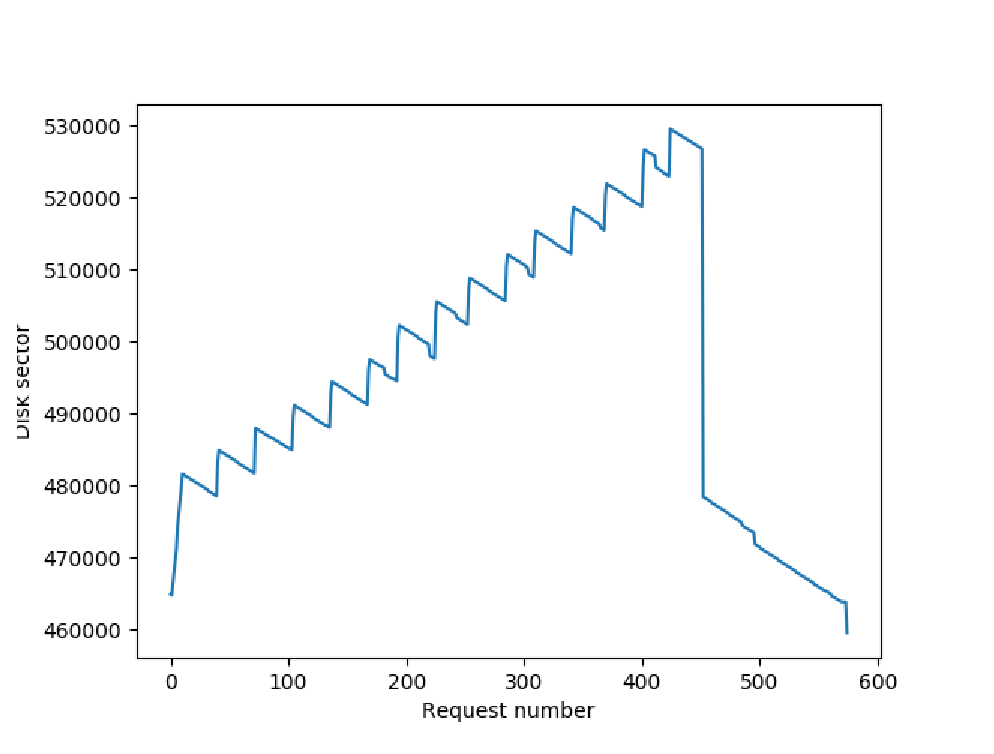
\includegraphics[width=\textwidth]{io_plot_2.eps}
  \caption{Graphing disk sector access during IO usage}
  \label{iograph}
\end{figure}

\subsubsection{What did you learn?}
\noindent We learned that disk I/O is not a difficult concept, but it does have some difficult (or at least difficult to find) implementation details.  For example, understanding where some of the Linux system calls were coming from took some research.  Understanding the scope of the problem was also difficult.  It would be easy to try to accomplish too much or too little and miss some portion of the assignment.
%--------------------------------------------------------------
\section{Dining Philosopher}
\subsection{Problem}
\noindent The problem states that we have 5 philosophers sitting around a round table and there are 5 chopsticks. in order for each philosopher to eat they have to have two chopsticks. Unfortunately there are only one chopsticks between each two philosophers. Philosophers can think, pickup left chopstick, pick up right chopstick, eat and put down both chopsticks. The problem asks us to think of a way where each philosopher eats and thinks without ending up starving.

\subsection{Solution}
\noindent The solution could be given by instructing each philosopher to follow the following operation:
\begin{itemize}
\item wait for a random amount of time
\item pickup the left chopstick if it is available
\item pickup the right chopstick if you have the left chopstick and right chopstick is available
\item if you have both chopsticks, eat for a random amount of time
\item put both chopsticks down
\item repeat
\end{itemize}

\subsection{Application}
\noindent The application is very similar to resource management. The resources that computer can provide are limited and processes need to use those resources. We can implement a similar algorithm for processes to use the resources available to them.

\subsection{Implementation}
\noindent In the implementation we follow exactly same pseudo-code as the solution subsection with an extra setup overhead:
\begin{itemize}
\item get the number of available threads
\item that number is the number of philosophers and chopsticks
\item run all of the threads as philosophers
\item each philosopher does the following:
	\begin{itemize}
	\item wait for a random amount of time
	\item pickup the left chopstick if it is available
	\item pickup the right chopstick if you have the left chopstick and right chopstick is available
	\item if you have both chopsticks, eat for a random amount of time
	\item put both chopsticks down
	\item repeat
	\end{itemize}
\end{itemize}

\subsection{Code}
\begin{minted}{c}
/*
	OSU - CS444
	Homework 1 - Dining Philosophers
	Behnam Saeedi, Levi Willmeth, Zhaoheng Wang
*/

#include <unistd.h>
#include "mt19937ar.c"
#include <pthread.h>
#include <ctype.h>
#include <stdio.h>
#include <stdlib.h>
#include <sys/types.h>
#include <sys/syscall.h>
#define MAXPHILOSOPHERS 5

pthread_mutex_t forks[MAXPHILOSOPHERS];

int think(int philosopher)
{
    // Waits for 1-20 seconds, inc
    unsigned int delay = genrand_int32() % 19 + 1;
    printf("%d is thinking for %d seconds.\n", philosopher, delay);
    sleep(delay);
    return delay;
}

int eat(int philosopher)
{
    // Waits for 2-9 seconds, inc
    unsigned int delay = genrand_int32() % 7 + 2;
    printf("%d has begun eating for %d seconds.\n", philosopher, delay);
    sleep(delay);
    return delay;
}

void get_forks(int philosopher)
{
    // The goal is not to block the forks unless I can pick up both of them.
    int prevFork = (philosopher - 1 + MAXPHILOSOPHERS) % MAXPHILOSOPHERS;
    int nextFork = philosopher;
    int leftHand;
    int rightHand;

    // printf("%d is ready for forks %d and %d.\n", philosopher, prevFork, nextFork);
    pthread_mutex_lock(&forks[nextFork]);
    pthread_mutex_lock(&forks[prevFork]);
    printf("%d has forks %d and %d.\n", philosopher, prevFork, nextFork);
}

void put_forks(int philosopher)
{
    // Puts down the forks
    int prevFork = (philosopher - 1 + MAXPHILOSOPHERS) % MAXPHILOSOPHERS;
    int nextFork = philosopher;
    pthread_mutex_unlock(&forks[nextFork]);
    pthread_mutex_unlock(&forks[prevFork]);
    printf("%d has set down forks %d and %d.\n", philosopher, prevFork, nextFork);
}


void *add_philosopher(void *n)
{
    unsigned int tid = pthread_self();
    int name = *((int *) n);
    free(n);
    printf("'I think, therefor I am!' - Philosopher %d.\n", name);
    // Just keep eating
    while(1){
        think(name);
        get_forks(name);
        eat(name);
        put_forks(name);
    }
}


int main(int argc, char **argv)
{
    // Create the philosophers
    pthread_t threads[MAXPHILOSOPHERS];

    printf("CS444 Homework 2: Dining Problem\n");
    for(int i=0; i<MAXPHILOSOPHERS; i++){
        int *arg = malloc(sizeof(*arg));
        *arg = i;
        pthread_create(&threads[i], NULL, add_philosopher, arg);
    }

    // Wait for all threads to finish
    for(int i=0; i<MAXPHILOSOPHERS; i++){
    		if(pthread_join(threads[i], NULL)){
    		fprintf(stderr, "Error absorbing philosopher.\n");
    		return 2;
      	}
    }
	  return 0;
}
\end{minted}
%--------------------------------------------------------------
\section{Work Log}
\noindent
\subsection{Hours}
\noindent All of the members of the group met every Monday, Wednesday and Friday from 2 to 4 for the purpose of group assignment. The team worked together in order to achieve the best possible solution for the Homework 2.
\subsection{Git Log}
\begin{table}[ht]
\centering
\caption{Git log for this assignment}
\label{GitLog}
\begin{tabular}{|
>{\columncolor[HTML]{999903}}l |l|l|l|}
\hline
\cellcolor[HTML]{329A9D}{\color[HTML]{FFFFFF} Hash} & \cellcolor[HTML]{329A9D}{\color[HTML]{FFFFFF} Author} & \cellcolor[HTML]{329A9D}{\color[HTML]{FFFFFF} Comment}    & \cellcolor[HTML]{329A9D}{\color[HTML]{FFFFFF} Date and time} \\ \hline
{\color[HTML]{FFFFFF} 8c41e84}                      & BeNsAeI                                               & added sstf-iosched.c                                      & 2017-05-04 13:23:53                                          \\ \hline
{\color[HTML]{FFFFFF} 3a7ee08}                      & Behnam Saeedi                                         & added the sstf-iosched.c                                  & 2017-05-04 10:33:01                                          \\ \hline
{\color[HTML]{FFFFFF} 4c22bc8}                      & Behnam Saeedi                                         & Merge branch 'master' of https://github.com/BeNsAeI/CS444 & 2017-05-04 10:31:57                                          \\ \hline
{\color[HTML]{FFFFFF} 088882c}                      & BeNsAeI                                               & added notes for lecture 8                                 & 2017-05-04 09:43:14                                          \\ \hline
{\color[HTML]{FFFFFF} 9b73121}                      & Levi Willmeth                                         & Switch to 5 philosophers and clean up unused struct.      & 2017-05-04 08:32:27                                          \\ \hline
{\color[HTML]{FFFFFF} 3ed4a02}                      & Levi Willmeth                                         & Switch to 5 philosophers and clean up unused struct.      & 2017-05-04 08:27:23                                          \\ \hline
{\color[HTML]{FFFFFF} 0e30ab9}                      & Behnam Saeedi                                         & it wokrs again!                                           & 2017-05-03 17:23:31                                          \\ \hline
{\color[HTML]{FFFFFF} ec7000f}                      & Behnam Saeedi                                         & Merge branch 'master' of https://github.com/BeNsAeI/CS444 & 2017-05-03 16:28:41                                          \\ \hline
{\color[HTML]{FFFFFF} aca83e9}                      & Behnam Saeedi                                         & dining dude works kinda                                   & 2017-05-03 16:27:39                                          \\ \hline
{\color[HTML]{FFFFFF} f977351}                      & Levi Willmeth                                         & pThreads solution to dining philosophers problem          & 2017-05-03 16:21:29                                          \\ \hline
{\color[HTML]{FFFFFF} 1df26c9}                      & Behnam Saeedi                                         & fixed qemu compile issue                                  & 2017-05-02 11:57:00                                          \\ \hline
{\color[HTML]{FFFFFF} 069f607}                      & BeNsAeI                                               & added notes and homework                                  & 2017-05-02 10:15:44                                          \\ \hline
{\color[HTML]{FFFFFF} 3cef067}                      & wangdaye123                                           & disable virtio qemu                                       & 2017-04-25 11:18:47                                          \\ \hline
{\color[HTML]{FFFFFF} bef1eef}                      & wangdaye123                                           & noop-iosched.c                                            & 2017-04-25 11:09:04                                          \\ \hline
{\color[HTML]{FFFFFF} 7a3c647}                      & wangdaye123                                           & hw2-Elevators                                             & 2017-04-25 11:00:51                                          \\ \hline
{\color[HTML]{FFFFFF} 947d202}                      & Levi Willmeth                                         & Remove cpp files because we submitted c files.            & 2017-04-25 10:34:25                                          \\ \hline
{\color[HTML]{FFFFFF} 82a3077}                      & Levi Willmeth                                         & Create HW2 directory and starter file                     & 2017-04-25 10:32:41                                          \\ \hline
{\color[HTML]{FFFFFF} bf2b478}                      & BeNsAeI                                               & Submission folder added                                   & 2017-04-20 11:06:49                                          \\ \hline
{\color[HTML]{FFFFFF} bd5dac7}                      & BeNsAeI                                               & Submission folder added                                   & 2017-04-20 11:04:32                                          \\ \hline
{\color[HTML]{FFFFFF} d4018fb}                      & Levi Willmeth                                         & Convert concurrency file from cpp to c.                   & 2017-04-20 10:55:41                                          \\ \hline
{\color[HTML]{FFFFFF} b5dab5b}                      & wangdaye123                                           & add file                                                  & 2017-04-19 18:50:50                                          \\ \hline
\end{tabular}
\end{table}

%--------------------------------------------------------------
\end{document}
